\chapter{Analiza problemu}
\thispagestyle{chapterBeginStyle}
\label{rozdzial1}
W niniejszym rozdziale omówiono problem redundancji oraz powiązanych pojęć, czyli detekcji i korekcji błędów. Opisano rownież zastosowane rozwiązania w ogólnym modelu systemu oraz relacje pomiędzy komponentami pracy, które wykorzystano w celu osiągnięcia jak największej niezawodności danych.

Implementowany projekt należy do grupy wirtualnych systemów plików, co pozwala na łatwe oraz intuincyjne montowanie w dowolnym miejscu dla wybranych katalogów, przez co w różnych miejscach nadrzędnego systemu plików mogą być zamontowane różne metody redundancji danych. Możliwe jest również wykorzystanie różnych nośników danych. 

Struktura systemu w założeniu jest rozłożona na warstwy. To znaczy, że każda opisywana funkcjonalność jak kodowanie czy odzyskiwanie plików jest niezależna od pozostałych i działa bez znajomości poprzedzających warstw. Takie rozwiązanie ułatwia dodawanie kolejnych funkcjonalności, lub rozszerzanie obecnych o nowe implementacje.

Założenia omawianego systemu:
\begin{itemize}
    \item Obsługa różnych rozwiązań redundancji
    \item Obsługa wielu kopii plików w celu zwiększenia niezawodności danych
    \item Wybór najodpowiedniejszej repliki do odczytu pliku 
    \item Synchronizacja już istniejących plików pomiędzy replikami 
	\item Obsługa podstawowych zachowań systemu plików:
		\begin{itemize}
			\item Odczyt oraz zapis danych
			\item Tworzenie oraz usuwanie plików
		\end{itemize}
	\item Detekcja błędów:
		\begin{itemize}
			\item Weryfikacja poprawności danych w pliku podczas odczytu
			\item Weryfikacja poprawności plików między kopiami 
		\end{itemize}
	\item Korekcja błędów:
		\begin{itemize}
			\item Zastosowanie kodów korekcyjnych
			\item Całkowite zastępowanie uszkodzonych plików poprawnymi kopiami
		\end{itemize}
    \item Wygoda użytkowania
\end{itemize}
\newpage
\section{System plików}
Do implementacji systemu plików wykorzystano interfejs FUSE, moduł w Unixowych jądrach pozwalający na tworzenie systemu plików w przestrzeni użytkownika. To rozwiązanie pozwala skupić się na tworzeniu pożądanej funkcjonalności, bez potrzeby schodzenia do poziomu jądra systemu. Projekt został zbudowany jako wirtualny system plików. Skupia się na translacji danych które otrzymuje, resztą zajmuje się nadrzędny system plików oraz moduł FUSE. 

\section {Redundancja danych}
Nadmiarowość zapisywanych informacji jest często stosowana w celu wykrycia uszkodzonych danych lub zabezpieczenia ich przed utratą po częściowym, czy całkowitym uszkodzeniu.
Redundancja danych stanowi najważniejsze zagadnienie rozważanej pracy. Zaproponowano kilka różnych rozwiżzań, aby przedstawić zakres możliwości systemu. Rozwiązania oparte są na macierzy RAID ze względu na ich skuteczność oraz mozliwość tworzenia kombinacji standardowych poziomów.

\subsection {RAID}
Redundant Array of Independent Disks \cite{RAID1} to metoda wirtualizacji przechowywania danych. Wykorzystuje wiele dysków i łączy je w logiczne jednostki pamięci. RAID jest stosowane do redundancji danych oraz lepszej wydajności, jednak w niniejszej pracy wydajność systemu nie będzie rozważana.  
RAID jest zbiorem schematów rozwiązań, które nazywane są poziomami. Na potrzeby pracy przedstawione zostaną wybrane poziomy, które wprowadzają różne metody redundancji.
\subsubsection{Poziom 0}
RAID-0 jako jedyny poziom RAID wprowadza zerową redundancję. Łączy przynajmniej dwa fizyczne nośniki danych w jeden dysk logiczny i w tej przestrzeni przeplata dane pomiędzy dyskami. Dane są dzielone na bloki o stałym rozmiarze. Poziom 0 w żaden sposób nie zapewnia niezawodności danych, jednak stanowi podstawę do innych poziomów. Wykorzystanie przeplotu danych na wiele dysków usprawnia operacje odczytu i zapisu wykonując je równolegle na wszystkich dyskach macierzy.
\begin{figure}[h!]
        \centering
        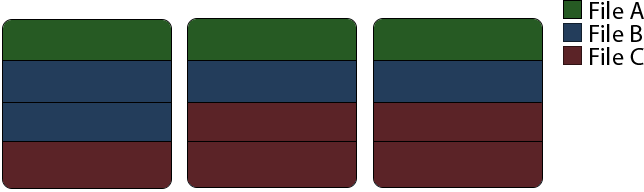
\includegraphics[scale=0.8]{raid-0.png}
        \caption{RAID-0 z trzema dyskami}
        \label{fig:raid0}
\end{figure}
\newpage
\subsubsection{Poziom 1}
RAID-1 działa na przynajmniej dwóch dyskach. Dane są zapisywane do wszystkich dysków, tworząc lustrzane odbicia. Z tego względu czas wykonywania dowolnych operacji jest równy sumie czasu trwania danej operacji na wszystkich dyskach, jednak możliwe jest przyśpieszenie działania. RAID-1 chroni przed utratą $(n-1)$ dysków macierzy, jednak przez to wymaga dużej ilości miejsca; dla $n$ dysków o rozmiarze $m$ potrzebne jest $n\times m$ wolnej przestrzeni.
\begin{figure}[h!]
        \centering
        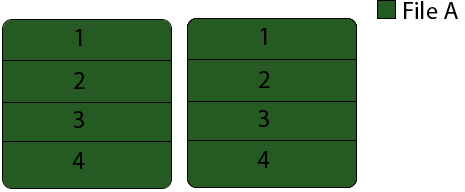
\includegraphics[scale=0.8]{raid-1.png}
        \caption{RAID-1 z dwoma dyskami}
        \label{fig:raid1}

\end{figure}

\subsubsection{Poziom 2}
Podobnie do RAID-0, dane są dzielone między dyskami. W przypadku poziomu drugiego, dane są dzielone na pojedyncze bity, a każdy bit jest zapisywany na kolejnym dysku. RAID-2 wykorzystuje kod Hamminga do korekcji występujących błędow, wszystkie bity kodu znajdują sie w odpowiednich dyskach i pozwalają na odzyskanie danych z jednego uszkodzonego dysku. 
\begin{figure}[h!tb]
        \centering
        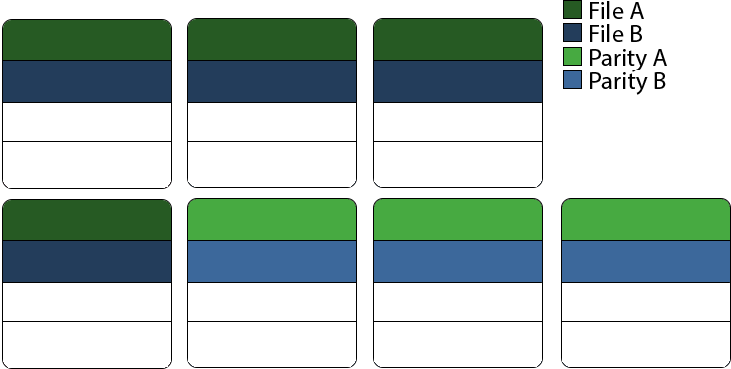
\includegraphics[scale=0.8]{raid-2.png}
        \caption{RAID-2 na siedmiu dyskach}
        \label{fig:raid2}
\end{figure}
\newpage
\subsubsection{Poziom 4}
Dane są dzielone na bloki ograniczonej wielkości i tak jak w przypadku poziomu 0, każdy blok jest zapisywany na kolejnym dysku. Do przechowywania danych służy $n-1$ dysków. Dla każdego rzędu zapisanych danych obliczany jest blok parzystości na osobnym dysku. Po uszkodzeniu jednego z dysków pojedynczy blok może zostać odzyskany.
\begin{figure}[h!]
        \centering
        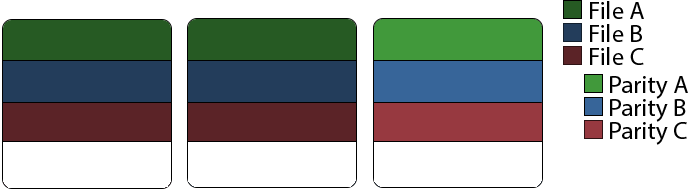
\includegraphics[scale=0.8]{raid-4.png}
        \caption{RAID-4 na trzech dyskach}
        \label{fig:raid4}

\end{figure}
\subsubsection{Poziom 5}
Dane są dzielone i bity parzystości są obliczane podobnie do poprzedniego poziomu, jednak bloki parzystości obliczane z $n-1$ bloków danych nie są zapisywane na dedykowanym dysku, tylko rozkładane równomiernie na wszystkich dyskach macierzy. Stąd dostępna pojemność to również $n-1$ i możliwe jest odzyskanie jednego uszkodzonego dysku.
\begin{figure}[h!]
        \centering
        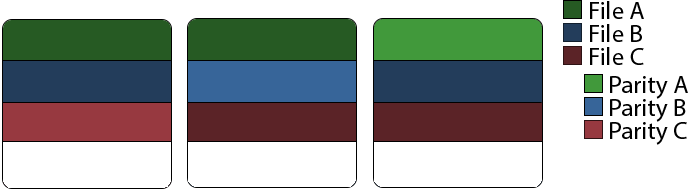
\includegraphics[scale=0.8]{raid-5.png}
        \caption{RAID-5 na trzech dyskach}
        \label{fig:raid5}
\end{figure}
\newpage
\subsection{Standardowe repliki systemu}
Repliki zostały zaprojektowane na podstawie poziomów RAID. Rozwiązania różną się 
między sobą sposobem wprowadzenia redundancji danych oraz podziału danych. 
System funkcjonuje z conajmniej jedną repliką, większa liczba replik oznacza większą redundantność. 
Poniżej opisano proponowane rodzaje replik oraz rozważono ich mocne i słabe strony. 
Repliki można podzielić na następujące kategorie:
\begin{itemize}
    \item Replika standardowa - dokonuje detekcji błędów w plikach, 
    jednak w przypadku wykrycia takiego błędu lub desynchronizacji z innymi replikami, 
    nie jest w stanie dokonać korekty błędów bez kopiowania danych z pozostałych replik.
    \item Replika korekcyjna - dokonuje zarówno detekcji, 
    jak i korekcji znalezionych błędów. 
    Jeśli korekta znalezionych błędów jest niemożliwa, zachowuje się 
    podobnie do repliki standardowej - desynchronizacja może zostać naprawiona wyłącznie 
    przy pomocy dodatkowych replik
\end{itemize}
Repliki korekcyjne rozszerzają funkcjonalność standardową, dlatego zostały omówione w późniejszej sekcji pracy. 

W przypadku trwałej awarii repliki takiej jak uszkodzenie dysku lub wystąpienie błędu bezpośrednio po próbie naprawy repliki, replika zostaje oznaczona jako nieaktywna i nie są podejmowane kolejne próby odczytu czy zapisu danych.
\subsubsection{Repliki Lustrzane (MR)}
Oparte na schemacie RAID-1 repliki tego typu stanowią lustrzane odbicie danych. 
Każdy plik występuje dokładnie raz we wszystkich replikach lustrzanych.
\begin{itemize}
        \item Naprawia błędy w innych replikach kopiując całe pliki
        \item Wszystkie dane zostają zamontowane w jednym miejscu. 
        W przypadku, kiedy dysk, na którym znajduje się replika, zostanie uszkodzony, 
        dane zostają utracone.
\end{itemize}

\begin{figure}[h!]
        \centering
        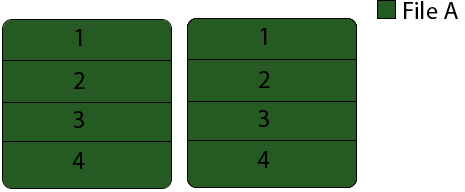
\includegraphics{raid-1.png}
        \caption{Dwie repliki lustrzane}
        \label{fig:raid1}
\end{figure}

Standardowa replika lustrzana nie jest w stanie naprawić znalezionych błędów. 
Jedynym rozwiązaniem jest zastąpić uszkodzone pliki w całości danymi z innej repliki. 
Repliki lustrzane z korektą błędów opisane w dalszej części pracy pozwalają 
naprawiać uszkodzone dane bez potrzeby przenoszenia plików pomiędzy replikami.
\subsubsection{Repliki Blokowe (BR)}
W replikach tego typu pliki są rozkładane na części i zapisywane w kolejnych katalogach 
będących odpowiednikiem dysków poziomu RAID-0. 
Tak samo katalogi mogą być rozmieszczone na różnych urządzeniach przechowujących. 
Każdy z katalogów może również być repliką, tworząc drzewo replik. 
Jedna część pliku nazywana jest dalej blokiem.
Rozkład danych jest możliwy na dwa sposoby:
\begin{itemize}
    \item Pliki podzielone na stałą liczbę bloków. 

            Zmiana wielkości pliku może powodować zmianę rozmiaru wszystkich bloków 
            danego pliku dla wyrównania wielkości, 
            lub jedynie tego bloku, do którego dane zostają dopisane. 
            W takim wypadku bloki nie są jednakowych rozmiarów. 
            Możliwe jest ograniczenie rozmiaru pojedynczego bloku, 
            tym samym ograniczając maksymalny rozmiar pliku. 
            Każde poddrzewo repliki ma dokładnie jeden blok pliku.
            \begin{figure}[h!]
                    \centering
                    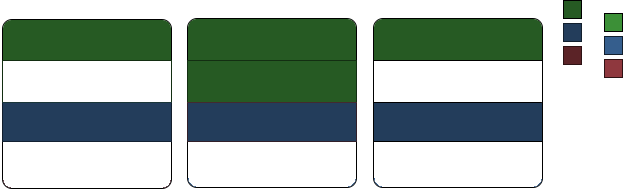
\includegraphics{BR-1.png}
                    \caption{Podział pliku na trzy nierówne bloki }
                    \label{fig:br1}
            \end{figure}
    \item Pliki podzielone na zmienną liczbę części o ograniczonych wielkościach

            Określony jest maksymalny dozwolony rozmiar dla pojedynczego bloku. 
            Przy przekroczeniu rozmiaru bloku, system tworzy kolejny w następnym katalogu 
            dopóki jest miejsce. W jednym poddrzewie repliki może znajdować się kilka bloków. 
            \begin{figure}[h!]
                    \centering
                    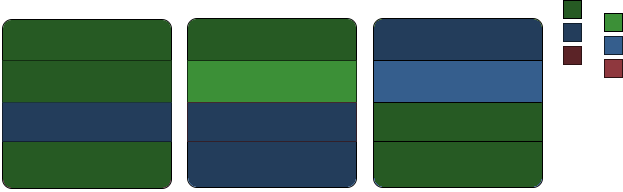
\includegraphics{BR-2.png}
                    \caption{Podzial pliku na wiele bloków ograniczonego rozmiaru}
                    \label{fig:br1}
            \end{figure}
 
\end{itemize}
Standardowe repliki blokowe nie są w stanie naprawić uszkodzonych plików, jednak taki podział danych wpłynie korzystnie na repliki korekcyjne i jest szczególnie przydatny dla wielu dysków. Jeśli replika blokowa działa na $n$ blokach, działa również po awarii na $n-1$ dyskach dla $n < 1$. Dodatkowo, replika blokowa rozszerzona o korekcję danych, może odzyskać utracony blok danych.

W przypadku awarii jednego z bloków repliki, replika jest nadal aktywna wtedy i tylko wtedy, jeśli odzyskano utracone dane i replika jest nadal w pełni funkcjonalna. Jeśli awarii uległ ostatni blok, a system nie może ustanowić nowej lokalizacji dla przynajmniej jednego bloku, replika zostaje uznana za nieaktywną.
\begin{itemize}
    \item Naprawia błędy innych replik kopiując jedynie częściowe pliki, jeśli to możliwe.
    \item Dane mogą zostać zamontowane w wielu miejscach. W przypadku uszkodzenia jednego dysku, reszta danych jest nadal dostępna.
\end{itemize}

\subsection{Podzial replik na warstwy}
W celu ułatwienia rozszerzalności działania replik, kolejne funkcje składają się na niezależne warstwy. W przypadku, kiedy użytkownik chce dodać nowe funkcje lub zmienić obecne, powinien być w stanie to zrobić bez konieczności zmian w niepowiązanych częściach systemu.


\section {Detekcja błędów}
    Wykrywanie błędów ma kluczowe znaczenie w działaniu opisywanego systemu. Po znalezieniu błędów plików, może nastąpić próba naprawienia, bądź zastapienia, uszkodzonych danych bez potrzeby ingerencji użytkownika. Wszystkie techniki detekcji błędów dodają kolejne bity do zapisu, tym samym zwiększając redundancję w systemie. Korzystanie z kontroli błędów niesie za sobą wykonywanie dodatkowych obliczeń nawet w trakcie podstawowych operacji na plikach, za każdym razem sprawdzając poprawność danych. Każda metoda ma kilka różnych rozkładów danych wynikających ze struktury replik. Niektóre metody detekcji przy odpowiednich warunkach mogą od razu dokonywać korekty wykrytych błędów, co zostało dokładniej opisane w kolejnym punkcie.
\subsection{Kod Hamminga}
Kod Hamminga \cite{Hamming} jest kodem korekcyjnym, wykrywa i naprawia błędy pojedynczego bitu. Chociaż szczegóły części korekcji zostają omówione w dalszej części pracy, kod Hamminga zostaje również wykorzystany do samej detekcji błędów dwóch bitów.
Odległość Hamminga $H_D$ mierzy liczbę miejsc, w których dwa ciągi o tej samej długości różnią się od siebie. Minimalna odległóść Hamminga dla kodu to najmniejsza odległość pomiędzy dowolnymi dwoma słowami z kodu. Dla kodów określa dwie ważne dla opisywanego problemu własności:
\begin{itemize}
        \item Kod  o minimalnej odległości $H_D = d$ może wykryć $(d-1)$ błędów
        \item Kod o minimalnej odległości $H_D = d$ może naprawić $\lfloor\dfrac{(d-1)}{2}\rfloor$ błędów
\end{itemize}
Kody Hamminga mają określoną minimalną odległość $H_D = 3$, więc z powyższych własności są w stanie wykrywać błędy do dwóch bitów.  W implementowanym systemie, kod Hamminga został wykorzystany zarówno jako metoda korekcji pojedynczego błędu w blokach określonego rozmiaru, jak i detekcji dwóch błędów.


\subsection{Sumy kontrolne}
    W celu weryfikacji, czy dane znajdujące się w pliku nie uległy niepożądanej zmianie, operacje wpływające na zawartość pliku obliczają sumę kontrolną. Niezgodność sumy zapisanej z sumą wyliczoną podczas próby odczytu oznacza wystąpienie błędu w danych pliku lub w samej sumie kontrolnej. Sumy kontrolne zapewniają spójność danych i są dołączane na koniec sprawdzanych danych, lub jako osobny plik. 
\subsubsection{Funkcje skrótu}
Funkcje skrótu są wykorzystywane do tworzenia krótkich, łatwych do zweryfikowania, podpisow. Obliczone sygnatury są dołączane do danych i chronią przed nieautoryzowanymi modyfikacjami danych. Funkcje skrótu zwracają kod stałego rozmiaru dla zbioru danych o dowolnej wielkości. Funkcja przechodzi ze zbioru ciągów dowolnej długości do zbioru kodów o stałej długości, więc może dojść do kolizji. Kolizja występuje kiedy dla dwóch różnych od siebie słów kodowanych funkcja zwraca tę samą wartość, uniemożliwiając wykrycie zmiany w zapisanych danych. Funkcja MD5 zostaąa wybrana do obliczania sygnatur plików.
\subsubsection{Kontrola parzystości}
Do zapisywanych danych można dopisać dodatkowe informacje o parzystości ustawionych bitów. Niech słowo kodowane $x \in (0,1)^n$ dla pewnego $n \ge 1$. Wtedy możliwe jest obliczenie $x_p = x_1 \oplus x_2 \oplus \cdots \oplus x_k$ dla $x_i$ takich, że $x_i = 1$. $x_p = 0$ jeśli liczba jedynek jest parzysta, $x_p = 1$ w przeciwnym wypadku. 

Niepożądana zmiana nieparzystej liczby bitów zostanie wykryta, ponieważ funkcja $xor$ przybierze wartość przeciwną poprzedniej. Zmiany parzystej ilości bitów pozostaną niezauważone.

\section {Korekcja błędów}
Kodowanie korekcyjne umożliwia wykrywanie i korygowanie określonych błędow. Kod korekcyjny jest zapisywany wraz z danymi, kodując wartości bitów podczas zapisu. W przypadku wystąpienia złych bitów podczas odczytu, kody korekcyjne mogą spróbować naprawić znalezione błędy bez wiedzy użytkownika.
\subsection{Kod Hamminga}
Wykorzystanie Kodu Hamminga zostało opisane, jednak przy korekcji błędów należy rozważyć pewną własność. Chociaż kodowanie pozwala na wykrycie dwóch błędów, w żaden sposób nie odróżnia błędów jednego bitu słowa od dwóch bitów. Z tego wynika, że jeśli system zawsze podejmie się próby korekcji słowa kodowanego po wykryciu błędu, słowo w niektórych przypadkach może zostać źle naprawione.
Dla zwiększenia skuteczności kodowanie, do kodu zostaje dodany dodatkowy bit parzystości. Kodowanie Hamminga z bitem parzystości zwiększa minimalną odległość $H_D$ = 4, co pozwala deterministycznie rozpoznać, czy znaleziono błąd jednego, czy dwóch bitów. Co więcej, jeśli kod Hamminga jest wykorzystywany jedynie do detekcji błędów, odległóść $H_D$ o wartości 4 oznacza, że dekoder może niezawodnie wykryć do trzech błędów.  
\subsection{Parzystość}
Kontrola parzystości pozwala odzyskać wartość pojedynczego bitu danych. Jeśli wartość pojedynczego bitu została utracona, informacja o ilości ustawionych bitœw w kodowanym ciagu wystarcza, aby rozpoznać wartość brakującego bitu.
\\
Korzystając z tej własności, tworzy się bloki bitów parzystości do osobnego pliku. W przypadku całkowitej utraty jednego bloku, obliczenia na pozostałych blokach pozwalają odzyskać dane.
\subsection{Repliki korekcyjne}
Dodanie metod korekcji błędów w replikach blokowych umożliwi odzyskiwanie całych bloków. Jeśli utracony blok posiadał jedynie kodowane dane, to traktując brakujący blok repliki jako zerowe bity, rozwiązania takie jak bity parzystości posiadają dostatecznie dużo informacji na temat danych, aby wyliczyć brakujące informacje. W takim wypadku repliki mogą zmienić lokalizację odzyskanego bloku danych lub dzielić dane na mniejszą ilość bloków. 

Ważny jest rozkład danych przy dodatkowej redundancji wynikającej z dodania do słów obliczonych kodów. W przypadku replik lustrzanych, możliwe są dwa rozwiązania:
\begin{itemize}
        \item Zapisywanie bitów kodu na końcu pliku
        \item Przeplatanie bitów kodu z kodowanymi danymi
\end{itemize}
Dla replik blokowych, ze względu na ich rozproszoną strukturę, przedstawiono następujące możliwości:
\begin{itemize}
        \item Zapisywanie bitów kodu w osobnym pliku na jednej replice
        \item Zapisywanie bitów kodu w osobnych plikach na kilku replikach
        \item Przeplatanie bitów kodu z kodowanymi danymi
\end{itemize}

\section {Synchronizacja replik}
Kiedy wirtualny system plików zostanie zamontowany, nie wiadomo jakie pliki znajdują się pod folderami wskazanymi jako repliki, zachodzi więc potrzeba synchronizacji plików pomiedzy replikami. Stąd repliki mogą znajdować się w przynamniej dwóch stanach. W przypadku wykrycia desynchronizacji, brakujące lub uszkodzone dane powinny zostać naprawione informacjami z pozostałych replik. Obslugiwane scenariusze desynchronizacji:
\begin{itemize}
    \item Brakujące dane w jednej z replik podczas montowania systemu pliku
    \item Różniące się między soba dane pomiędzy replikami podczas montowania systemu plików
\end{itemize}
Kiedy następuje próba odczytu brakującego pliku w wybranej replice, system może sprawdzić obecność tego pliku w pozostałych miejscach. Jeśli znaleziono, następuje synchronizacja replik z brakującymi danymi. 

Jeśli podczas synchronizacji replik system wykryje różne dane w kopiach tego samego pliku i wszystkie kopie zostaną oznaczone jako niepoprawne, występuje konflikt. Taki konflikt może rozwiązać jedynie użytkownik.  

\section {Sposób użytkowania}
Działanie systemu, takie jak podział na repliki czy podział plików na bloki, powinno być niewidoczne dla użytkownika. Detekcja, czy naprawa błędów oraz synchronizowanie replik odbywa się w tle.

Użytkownik jest stale informowany o zachodzących procesach, a system zatrzymuje działanie wyłącznie kiedy nie może dalej samodzielnie operować. Konflikty podczas synchronizacji są rozwiązywane przez użytkownika, który wybiera najlepszą opcję na podstawie zawartości plików wywołujących konflikt.

